% Generated from ../chapters/02-how-complex-systems-become-stable.md
\chapter{How Complex Systems Become Stable}\label{chapter-2-how-complex-systems-become-stable}

Before speaking about healthy attractors, we need to understand what an attractor is and why the idea is useful.

A system is anything whose state can change over time. The state of a pendulum can be described by its angle and velocity. The state of a population may include the number of organisms and available resources. The state of a body is vastly larger: positions, forces, chemical concentrations, electrical potentials, cell identities, neural activity, beliefs, and environmental relations.

The set of all states a system could occupy is called its \textbf{configuration space} or, when velocities and other dynamic variables are included, its \textbf{state space}. We cannot draw the full state space of a person. It has too many dimensions. But we can reason about its geometry.

Imagine a landscape of hills and valleys. A ball placed on a slope tends to roll downhill. The bottom of a valley is a stable state: small disturbances move the ball, but it returns. In dynamical-systems language, the valley represents a basin of attraction and the bottom represents an attractor.

The analogy becomes useful when behavior is repetitive. A person with chronic pain may repeatedly return to a guarded movement pattern. A society may return to familiar institutions after political shocks. An ecosystem may settle into one of several stable regimes. A neural network may converge on a pattern representing a memory. The material differs, but the abstract question is similar: which states are stable, and what determines transitions between them?

Physical energy landscapes provide the clearest intuition. Molecules often occupy local energy minima. A reaction may have a lower-energy product available, yet remain trapped because it must first cross an activation barrier. Heat, a catalyst, or another perturbation can make the transition possible. Protein folding is frequently described through a landscape containing many possible conformations and a smaller set of stable folds.

Living systems complicate the picture. They are open systems that consume energy and maintain themselves far from thermodynamic equilibrium. Their landscapes are not fixed. Cells change the environment that changes them; organisms alter their own constraints; learning reshapes which patterns are easy to revisit. An attractor in biology is therefore not merely a passive low-energy state. It may be an actively maintained pattern.

This leads to an important distinction between \textbf{stability} and \textbf{health}. A pattern can be stable because the system repeatedly reinforces it, not because it is desirable. Chronic inflammation, metabolic disease, learned helplessness, and a pain-guarding loop can all become stable. Stability tells us that a pattern reproduces itself. It does not tell us that the pattern serves the whole organism.

A transition requires enough change to make the old attractor lose its grip or to make another attractor more accessible. In bodily practice, relaxation and challenge may play complementary roles. Relaxation can release constraints that keep the system confined to one narrow solution. Challenge can supply the demand that makes a different solution necessary. Relaxation without challenge may produce comfort without adaptation; challenge without relaxation may deepen the old compensation.

\begin{figure}
\centering
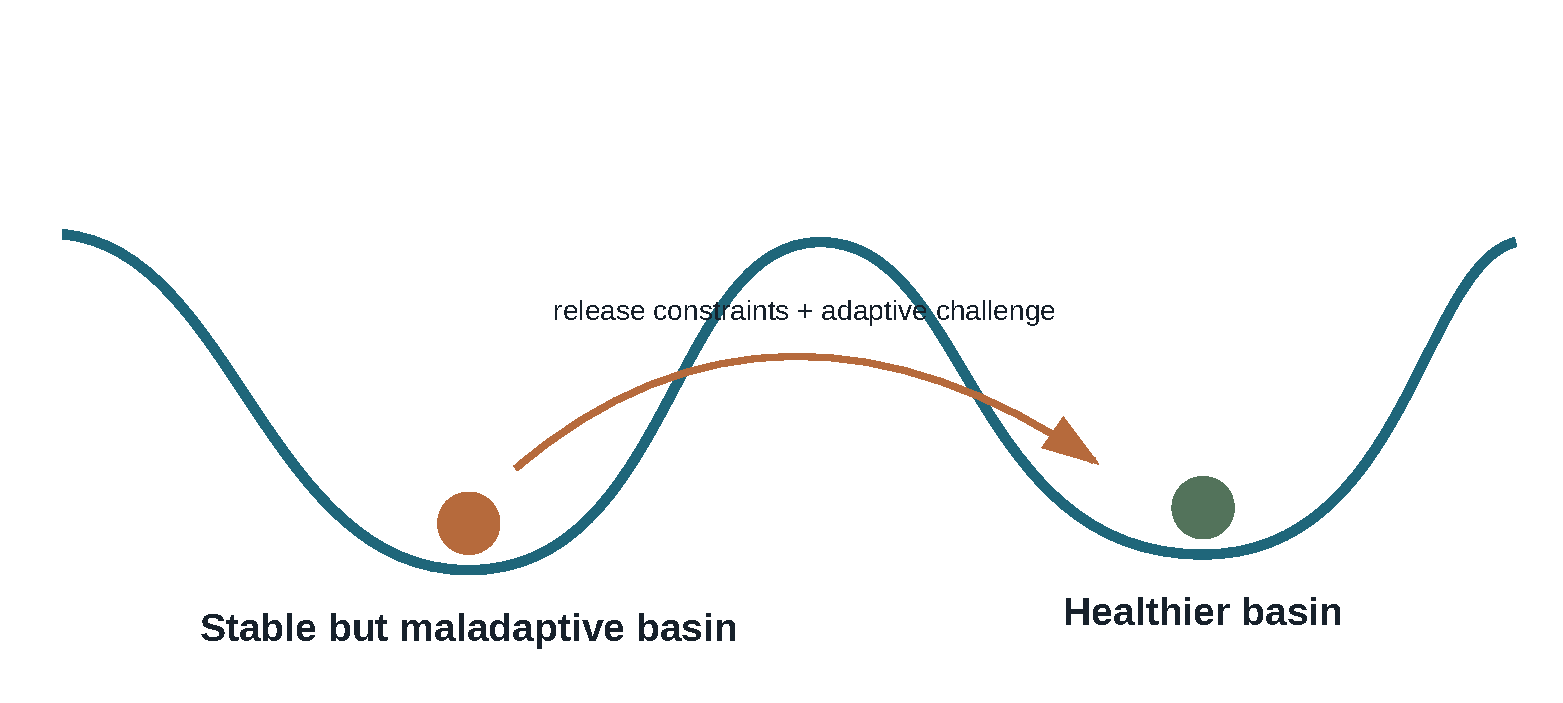
\includegraphics[width=0.88\textwidth,height=.68\textheight]{../figures/attractor-landscape.pdf}
\caption{A system may be trapped in a stable but maladaptive local minimum. Relaxation can lower constraints and progressive challenge can help it cross into a healthier basin.}\label{fig:attractor}
\end{figure}

The figure is conceptual, not a literal measurement of bodily energy. Its value is explanatory. It helps us ask what variables define the state, which feedbacks deepen a basin, what perturbation could enable escape, and whether a new state remains stable after the intervention ends.

Dynamical-systems approaches have been applied to motor coordination, neural activity, ecology, physiology, and resilience. The concept of critical slowing down, for example, describes how a system near a transition may recover more slowly from disturbances \autocite{scheffer2009early}. In clinical gerontology, resilience is increasingly studied through recovery trajectories rather than static measurements alone \autocite{gijzel2017resilience}.

The practitioner need not calculate a high-dimensional landscape. But a scientist or clinician can operationalize the idea: measure how quickly gait, heart rate, glucose, cognition, or muscle activation returns after a standardized perturbation. A healthier organism may be distinguished not only by its resting state but by the shape of its return.
